\documentclass[11pt,a4paper]{article}

\usepackage[T1]{fontenc}
\usepackage[utf8]{inputenc}
\usepackage[norsk]{babel}
\usepackage{lmodern}
\renewcommand{\familydefault}{\sfdefault}
\usepackage[a4paper,top=25mm,bottom=25mm,left=27mm,right=27mm]{geometry}
\usepackage{microtype}
\usepackage{amsmath}
\usepackage{booktabs}
\usepackage{tabularx}
\usepackage{graphicx}
\usepackage{xcolor}
\usepackage{tikz}
\usetikzlibrary{arrows.meta,positioning}
\usepackage{pgfplots}
\pgfplotsset{compat=1.18}
\usepackage{csquotes}
\usepackage[backend=biber,style=numeric,sorting=none,maxbibnames=6]{biblatex}
\addbibresource{references.bib}
\renewcommand*{\mkbibnamefamily}[1]{#1}
\renewcommand*{\mkbibnamegiven}[1]{#1}
\renewcommand*{\mkbibacro}[1]{\MakeUppercase{#1}}
\usepackage{hyperref}
\usepackage{fancyhdr}
\usepackage{enumitem}
\usepackage{caption}
\usepackage{placeins}
\usepackage{titlesec}

\definecolor{reportblue}{HTML}{17365D}
\definecolor{reportteal}{HTML}{007F82}
\hypersetup{
  colorlinks=true,
  linkcolor=reportblue,
  citecolor=reportblue,
  urlcolor=reportteal,
  pdftitle={Bergen Traffic Predictor},
  pdfauthor={Eirik Karlsen Ingebrigtsen, Jone Kjellstadli, Håvard Thu}
}
\setlength{\parindent}{0pt}
\setlength{\parskip}{0.65em}
\setlength{\emergencystretch}{2em}
\setcounter{tocdepth}{2}
\setlist{nosep,leftmargin=1.5em}
\captionsetup{font=small,labelfont=bf}
\titleformat{\section}{\normalfont\LARGE\bfseries}{\thesection}{0.9em}{}
\titleformat{\subsection}{\normalfont\large\bfseries}{\thesubsection}{1.15em}{}
\titlespacing*{\section}{0pt}{2.2ex plus 0.5ex}{1.0ex}
\titlespacing*{\subsection}{0pt}{2.0ex plus 0.4ex}{0.8ex}
\AtBeginBibliography{\small}
\setlength{\bibitemsep}{0.25\baselineskip}
\pagestyle{fancy}
\fancyhf{}
\fancyfoot[C]{\thepage}
\renewcommand{\headrulewidth}{0pt}
\renewcommand{\sectionmark}[1]{}

\newcommand{\groupmembers}{\texttt{Eirik Karlsen Ingebrigtsen, Jone Kjellstadli, Håvard Thu}}
\newcommand{\reportdate}{\today}

\begin{document}

\begin{flushright}
  DAT158 Innlevering 2
\end{flushright}
\vspace{0.5em}
{\fontsize{27}{32}\selectfont Bergen Traffic Predictor\par}
\vspace{0.45em}
{\large \groupmembers\par}
{\large \reportdate\par}
\vspace{1.5em}

{\small
\textbf{Kort sammendrag.} Bergen Traffic Predictor predikerer trafikkvolumet ved Danmarks plass én time frem i tid. Prosjektets opprinnelige mål var å undersøke om værdata kunne forbedre prediksjonene, men eksperimentene viste at historiske værdata fra Frost ikke ga bedre resultater. Den endelige modellen bruker derfor historiske trafikkdata fra Statens vegvesen samt kalenderinformasjon, blant annet om helligdager. Modellen ble sammenlignet med en baseline som bruker trafikkvolumet på samme tidspunkt én uke tidligere. På testsettets 4 343 observasjoner oppnådde modellen en MAE på 108,81 kjøretøy per time, mot 211,79 for baselinen. Sluttproduktet er en lokal Streamlit-demonstrasjon for ett målepunkt.
\par}

\section{Beskriv problemet}

\subsection{Omfang}

Bergen Traffic Predictor estimerer hvor mange kjøretøy som passerer ett bestemt
trafikkregistreringspunkt i løpet av neste time. Punktet er Danmarks plass med ID
\texttt{14630V805616}. Hver modellrad representerer et tidspunkt $t$, mens
\emph{target} er observert trafikkvolum ved $t+1$. Oppgaven er dermed
\emph{supervised regression} og en kortsiktig tidsserieprognose.

Prosjektets opprinnelige hypotese var at historiske værdata fra MET Norways Frost
API kunne forbedre prediksjonene. Værvariantene tapte i kronologisk validering, så
sluttmodellen ble værfri som følge av eksperimentene.

En videreutviklet løsning kan gi trafikkplanleggere og analytikere et anslag for
belastningen ved punktet. Den manuelle referansen er trafikken på samme klokkeslett
én uke tidligere, eventuelt justert skjønnsmessig for helg eller ferie. Dette er
prosjektets baseline. Maskinlæring er relevant fordi trafikken varierer med time,
ukedag og kalenderhendelser, og fordi trafikkverdier fra flere tidligere
tidspunkter kan samvirke ikke-lineært. Modellen mangler likevel informasjon om blant annet ulykker,
vegarbeid og arrangementer.

Prognosen kan brukes til å oppdage avvik fra et normalt ukemønster eller som ett av
flere grunnlag for planlegging. Studentprosjektet har imidlertid ikke undersøkt
faktisk beslutningsbruk, brukertall eller økonomisk gevinst. Løsningen demonstrerer
derfor teknisk gjennomførbarhet, ikke dokumentert nytte eller lønnsomhet i drift.

Avgrensningen til ett punkt og én times horisont gjør dataløpet og evalueringen
entydig. Modellen sier ikke noe om reisetid, kølengde eller retning og kan ikke
overføres direkte til andre målepunkter med andre trafikkmønstre.

Figur~\ref{fig:pipeline} viser systemgrensen. Traffic Data API leverer aggregerte
timesmålinger med kvalitetsparametere \cite{vegvesen-traffic-api}. Prosjektet
normaliserer serien, bygger modellvariabler fra eksakte tidspunkter, trener modellen
og bruker den i Streamlit. Trening og app deler feature-kode, mens datakvalitet og
publiseringsforsinkelse avgjør om en prognose kan lages.

\begin{figure}[htbp]
  \centering
  \resizebox{\textwidth}{!}{\begin{tikzpicture}[
  node distance=5.5mm and 5.5mm,
  stage/.style={draw=black!55, rounded corners=1.5pt, fill=black!3,
    minimum height=10mm, text width=27mm, align=center, font=\small},
  arrow/.style={-{Latex[length=2mm]}, semithick, draw=black!70}
]
\node[stage] (api) {Traffic Data API\\timevolum};
\node[stage, right=of api] (prepare) {Validering og\\komplett timeakse};
\node[stage, right=of prepare] (features) {Kalender og eksakte\\lag på tidspunkt};
\node[stage, right=of features] (model) {Frosset HGB\\og metadata};
\node[stage, right=of model] (app) {Lokal\\Streamlit-app};
\draw[arrow] (api) -- (prepare);
\draw[arrow] (prepare) -- (features);
\draw[arrow] (features) -- (model);
\draw[arrow] (model) -- (app);
\end{tikzpicture}
}
  \caption{Implementert dataløp fra offentlige trafikkdata til lokal demonstrasjon.}
  \label{fig:pipeline}
\end{figure}
\FloatBarrier

Prosjektet regnes som vellykket dersom en lekkasjesikker modell slår
forrige-uke-baselinen på en senere, urørt periode, kan bygges reproduserbart og gir
enten prognose eller tydelig feilmelding. Flerårige timedata og HGB-modellen kan
håndteres på en vanlig bærbar datamaskin. Den viktigste ressursen er
utviklingsarbeid til datavalidering, lekkasjekontroll, evaluering og integrasjon.
En produksjonsløsning ville i tillegg krevd driftsansvar, overvåking og rutiner for
godkjenning av nye modellversjoner.

\subsection{Metrikker}

Hovedmetrikken er gjennomsnittlig absolutt feil, MAE,

\begin{equation}
  \operatorname{MAE}=\frac{1}{n}\sum_{i=1}^{n}|y_i-\hat{y}_i|.
\end{equation}

MAE måles i kjøretøy per time og kan tolkes direkte. RMSE rapporteres som støttemål
fordi kvadreringen gir større utslag for enkelte store feil:

\begin{equation}
  \operatorname{RMSE}=\sqrt{\frac{1}{n}\sum_{i=1}^{n}(y_i-\hat{y}_i)^2}.
\end{equation}

Modell og baseline måles på de samme prognoseradene. Vi rapporterer også antall
prediksjoner og feil etter time og ukedag. Felles rader hindrer at ulik
tilgjengelighet av historiske trafikkverdier gir forskjellige evalueringsutvalg.
Programvaren testes for reproduserbar bygging, modellasting, manglende historiske
trafikkverdier, API-feil og tidssoner. Svartid,
oppetid og brukertilfredshet er ikke målt i den lokale demonstrasjonen.

\section{Data}

\subsection{Kilde, periode og labels}

Trafikkdata hentes fra Statens vegvesens åpne Traffic Data API, som inneholder
aggregerte registreringer fra offentlige veger \cite{vegvesen-traffic-portal}. Uttrekket
dekker 1. januar 2022 til 1. juli 2026 i lokal tid og gjelder feltet
\enquote{Totalt} ved punkt \texttt{14630V805616}. Den normaliserte timeaksen har
39 407 timer. Av disse har 38 956 observert trafikkvolum og 451 mangler verdi. Perioden
2022--2025 har 35 064 timer, 34 613 observasjoner og alle de 451 manglene. Den
reserverte perioden 2026 H1 har 4 343 observerte timer og ingen mangler.

Figur~\ref{fig:danmarks-plass-kart} gir geografisk kontekst for
registreringsområdet.

\begin{figure}[tbp]
  \centering
  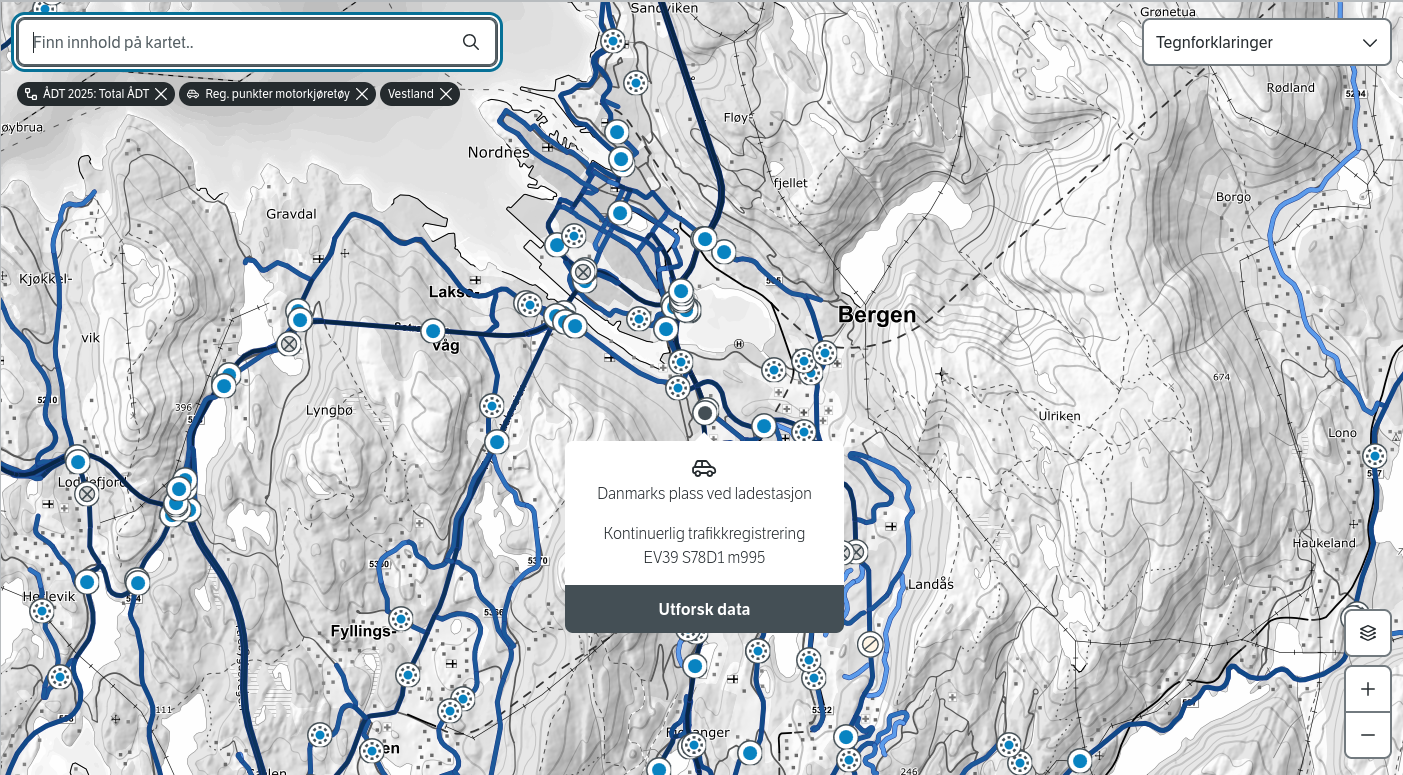
\includegraphics[width=0.94\textwidth]{figures/danmarks_plass.png}
  \caption{Geografisk oversikt over registreringsområdet ved Danmarks plass i
  Statens vegvesens Trafikkdataportal. Skjermbildet viser portalens kartvisning
  og valgte målested.}
  \label{fig:danmarks-plass-kart}
\end{figure}

Det opprinnelige API-uttrekket inneholder 39 025 rader. Kvalitetsrapporten markerer
69 av dem som ugyldige fordi volum mangler, men finner ingen dupliserte timestamps.
Når datasettet reindekseres til alle forventede UTC-timer, blir både disse radene og
timer uten API-rad stående som ukjente verdier. Forskjellen mellom rått radantall og
39 407 timer på den komplette aksen er derfor forventet og dokumentert, ikke et tap
som oppstår under behandling.

API-resultatet lagres først som rå CSV sammen med kilde, hentetidspunkt, punkt-ID,
periode og radantall. Det prosesserte datasettet får en sidecar-fil med SHA-256 for
råfilen, kvalitetsrapport og kolonneliste. Rådata, prosesserte data og
modellartefakter er utelatt fra Git, men kan gjenskapes med \texttt{make
build-app-model}. Denne kommandoen henter hele perioden, bygger datasettet og trener
sluttmodellen.

Labelen oppstår uten manuell annotering: for en feature-rad ved $t$ slås
\texttt{traffic\_volume} ved nøyaktig $t+1$ opp som
\texttt{target\_traffic}. Trafikkmåleren er dermed både datakilde og fasit. Dette gir
konsistente enheter, men ikke nødvendigvis en feilfri sannhet; sensorfeil og
ufullstendig dekning kan fortsatt påvirke både features og labels. API-ets
kvalitetsinformasjon lagres i rådataene, mens denne prosjektversjonen primært bruker
tilstedeværelse, gyldig timestamp og ikke-negativt volum som valideringskrav.

\subsection{Rensing og målegap}

Innlest tid konverteres til tidssonebevart UTC, sorteres og kontrolleres for ugyldige
og dupliserte tidspunkter. Kalenderinformasjon beregnes etter konvertering til
\texttt{Europe/Oslo}. Denne arbeidsdelingen bevarer entydige tidspunkt gjennom
sommertid og vintertid samtidig som time og dato får riktig lokal betydning.

Det finnes to dokumenterte målegap: 67 timer fra 4. juni 2022 kl. 21 til 7. juni
kl. 15, og 384 timer fra 2. oktober 2024 kl. 10 til 18. oktober kl. 09, alle tider i
\texttt{Europe/Oslo}. Pipelinen oppretter en komplett timeakse og lar disse 451
verdiene stå som manglende. De blir ikke satt til null, interpolert eller erstattet.
Null ville betydd observert fravær av trafikk, mens en manglende verdi betyr at
volumet er ukjent. Minimum og maksimum blant observerte timer i hele datasettet er
henholdsvis 40 og 4 235 kjøretøy; ingen observerte timer er null.

Den innledende EDA-en viste et tydelig døgn- og ukemønster. For 2022--2025 var
gjennomsnittet høyest kl. 15 med 3 426 kjøretøy per time og lavest kl. 03 med 185.
Helgesnittet var 1 275, som var 32,5 prosent lavere enn hverdagssnittet på 1 889.
Disse mønstrene begrunner kalenderfeatures og den ukentlige baselinen, men de brukes
ikke som en alternativ fasit. Volumfordelingen alene sier heller ikke om en høy verdi
er normal for en bestemt dato.

Alle lag og targets hentes ved eksakt timestamp, aldri ved radforskyvning. Hvis en
feature krever $t-24$ og denne timen ligger i et målegap, blir featuren manglende selv
om forrige tilgjengelige rad finnes 25 timer tilbake. Modellrader med manglende
nødvendig trafikklag eller target fjernes før trening og evaluering. Dette er et
dokumentert utvalg, ikke imputering, og hindrer at observasjoner flyttes over hull i
serien.

\subsection{Feature engineering}

Sluttmodellen bruker 14 features. Seks beskriver lokal kalender: time, ukedag,
måned, helg samt sinus og cosinus av time. Fem deterministiske indikatorer markerer
offentlig helligdag, dag før og etter helligdag, jul- og nyttårsperioden og 17. mai.
De tre numeriske traffic lag features er observert volum ved nøyaktig $t-24$, $t-48$ og
$t-168$. Alle er kjent eller kan konstateres som manglende ved prognosetidspunktet.
Den tree-based sluttmodellen krever ingen scaling.

Sinus og cosinus gjør at kl. 23 og kl. 00 ligger nær hverandre i
feature-representasjonen. Helligdagsindikatorene beregnes fra kalenderen og krever
ingen observerte fremtidsdata. Trafikklagene følger derimot absolutte tidsforskjeller
i UTC. Dermed endres ikke den faktiske avstanden ved overgang mellom sommer- og
vintertid, selv om det lokale klokkeslettet kan være annerledes.

Værdataene ble hentet fordi prosjektets opprinnelige hypotese var at weather features
kunne forbedre prediction utover det historisk trafikk alene ga. Historiske
observasjoner kom fra MET Norways Frost API for Bergen--Florida (SN50540). Frost gir
tilgang til arkiverte observasjoner og krever kilde,
referansetid og element i forespørselen \cite{frost-howto}. Temperatur og nedbør
dekket 35 016 av 35 064 timer i 2022--2025, mens vind dekket 34 458. Prosjektet
brukte konservative weather lag features fordi \texttt{referenceTime} beskriver
observasjonstid, ikke publiseringstid \cite{frost-time-concepts}. Både de direkte
weather lag features og en senere avledet weather feature-pakke ga svakere
validation enn traffic-only model. Det sentrale forsøket på å forbedre modellen med
vær lyktes dermed ikke, og Frost inngår derfor ikke i sluttmodellen eller appen.

\subsection{Personvern og etikk}

Datasettet inneholder aggregerte passeringstall per time, ikke kjøretøy- eller
personidentifikatorer. Personvernrisikoen er derfor lav. Den viktigste etiske
risikoen er feilaktig bruk: ett registreringspunkt representerer ikke all trafikk på
Danmarks plass eller Bergen, og en prognose kan være misvisende ved hendelser som
modellen ikke kjenner. Appen oppgir derfor punkt-ID, datakilde og begrensning. En
senere operativ løsning bør i tillegg dokumentere datalisens, tilgjengelighet,
sensorendringer og hvem som har ansvar for beslutninger som støttes av prognosen.

\section{Modellering}

\subsection{Fra værhypotese til frozen candidate}

Utviklingen fulgte en kronologisk ML lifecycle med værhypotesen som utgangspunkt.
Målet var å undersøke om weather features kunne gi lavere feil enn modeller basert
på historisk trafikk. Først ble forrige-uke-prediksjonen etablert som kontroll. For
en forecast med target $t+1$ bruker baselinen observasjonen ved
$(t+1)-168=t-167$, altså samme target-time én uke tidligere. En lineær regresjon og
en \texttt{HistGradientBoostingRegressor} (HGB) ble deretter trent med kalender og
traffic lag features ved $t-1$, $t-2$, $t-24$ og $t-168$. HGB er en
histogram-based gradient boosting model for tabulære data. På validation i 2024
fikk lineær regresjon MAE 322,45, HGB 103,28 og baselinen 200,78. HGB ble derfor
valgt og oppnådde MAE 106,22 på 2025-testen.

Sammenligningen brukte 8 231 felles rader i 2024 og 8 760 i 2025. Modellen ble først
tilpasset på 2022--2023 for validation. Etter valg ble HGB trent på training- og
validation-data samlet før den ene målingen på 2025-testen. Denne rekkefølgen skiller
mellom model selection og å anslå generalization error. Dersom 2025 hadde blitt brukt til
å endre features etter hver måling, ville perioden gradvis blitt en ny
validation period og sluttresultatet for optimistisk.

Videre analyse viste at store feil ofte sammenfalt med helligdager og høytider.
Deterministiske norske kalenderindikatorer ble derfor vurdert med tre expanding
folds i 2022--2023. Gjennomsnittlig CV-MAE ble 119,69 med indikatorene og 120,03
uten. Deretter ble den opprinnelige værhypotesen testet direkte. En raw weather model
tapte mot traffic-only model på felles 2024-rader, med MAE 106,73 mot 103,41. En
forhåndsdefinert weather feature-pakke med blant annet akkumulert nedbør og
sesongavvik for temperatur og vind tapte senere alle tre CV-foldene: 124,43 mot
119,69. Vær ga altså ingen dokumentert forbedring i noen av de to forsøkene og ble
forkastet før sluttmodellen ble bestemt.

Den første frozen calendar HGB-en oppnådde MAE 102,35 på 2025, men krevde de ferske
lag features $t-1$ og $t-2$. Traffic Data API kan publisere timeaggregater med forsinkelse,
så modellen var lite egnet til en reell neste-time-forespørsel. Prosjektet definerte
derfor tre små, latency-robust lagpakker på forhånd: $(24,168)$, $(24,48,168)$ og
$(24,168,336)$. Alle brukte de samme calendar feature-typene og HGB med fast
\texttt{random\_state=42}. Gjennomsnittlig CV-MAE i 2022--2023 ble henholdsvis
134,88, 133,77 og 135,80. Pakken $(24,48,168)$ ble fryst som
\texttt{traffic-hgb-latency-robust-v1}.

Den latency-robust modellen er ikke kandidaten med lavest tidligere 2025-MAE; den
løser et annet programvarekrav. Ved å fjerne $t-1$ og $t-2$ kan appen lage en
prognose selv om de nyeste aggregatene ikke er publisert. Kostnaden er at modellen
mister informasjon om den umiddelbare trafikkutviklingen. Kandidatlisten ble holdt
liten for å begrense tilpasning til CV-foldene, og ingen hyperparameters ble valgt
fra 2026-resultatet.

\subsection{Kronologisk evaluering}

Random splitting ville blandet fortid og fremtid og gitt en misvisende vurdering av
tidsserien. Prosjektet brukte derfor time-series cross-validation der hver validation
period ligger etter training period. Model selection brukte expanding training
windows med validation i 2022 H2, 2023 H1 og 2023 H2. Perioden 2025 var allerede
brukt som test set for en tidligere modell og ble derfor låst for videre valg. Etter
at den latency-robust kandidaten var frozen, ble den trent på 2022--2025 og evaluert
én gang på det nye test set-et 2026 H1. Sluttresultatet ble ikke brukt til ny tuning.

Tabell~\ref{tab:final-results} sammenligner modell og baseline på nøyaktig de samme
4 343 radene. Modellen reduserer MAE med 102,98 kjøretøy per time, tilsvarende 48,6
prosent relativt til baselinen. RMSE er også vesentlig lavere, men ligger over MAE
fordi enkelte timer har store feil.

\begin{table}[htbp]
  \centering
  \caption{Sluttevaluering på den tidligere ubrukte perioden 2026 H1.}
  \label{tab:final-results}
  \begin{tabularx}{\textwidth}{Xrrr}
    \toprule
    Modell & MAE & RMSE & Rader \\
    \midrule
    Latensrobust HGB & 108,81 & 161,85 & 4 343 \\
    Forrige uke & 211,79 & 454,47 & 4 343 \\
    \bottomrule
  \end{tabularx}
\end{table}

\subsection{Feature importance}

For å undersøke hva den valgte modellen faktisk bygger prediction på, ble
permutation feature importance beregnet med MAE som scoring. Modellen ble trent på
nytt i hver av de tre kronologiske CV-foldene, og hver feature ble permutert 30
ganger på foldens validation-data. Figur~\ref{fig:feature-importance} viser
gjennomsnittlig økning i MAE; en høy positiv verdi betyr at modellen mister mye
predictive performance når sammenhengen til target brytes. Analysen ble utført etter
at kandidaten var frozen og ble ikke brukt til å endre modell eller features.

\begin{figure}[htbp]
  \centering
  \begin{tikzpicture}
    \begin{axis}[
      xbar,
      width=0.82\textwidth,
      height=8.4cm,
      xlabel={Økning i MAE (kjøretøy/time)},
      table/col sep=comma,
      ytick=data,
      yticklabels from table={figures/feature_importance.csv}{label},
      y dir=reverse,
      xmajorgrids=true,
      grid style={black!12},
      axis line style={black!55},
      tick style={black!55},
      bar width=5pt,
      enlarge y limits=0.035,
      error bars/x dir=both,
      error bars/x explicit
    ]
      \addplot[fill=reportblue!75, draw=reportblue]
        table[
          x=mean_delta_mae,
          x error=std_delta_mae,
          y expr=\coordindex,
          col sep=comma
        ]{figures/feature_importance.csv};
    \end{axis}
  \end{tikzpicture}
  \caption{Cross-validated permutation feature importance for den frozen
  latency-robust modellen. Error bars viser standardavvik over 90 permutasjoner
  per feature, fordelt på tre validation-folds.}
  \label{fig:feature-importance}
\end{figure}

Størst importance fikk \texttt{traffic\_168h\_ago} med en gjennomsnittlig
MAE-økning på 394,64, etterfulgt av \texttt{hour\_cos} med 366,88,
\texttt{traffic\_24h\_ago} med 223,15 og \texttt{day\_of\_week} med 182,21.
Resultatet viser at modellen særlig støtter seg på ukerytme, døgnsyklus og trafikken
ett døgn tidligere.

Resultatet må tolkes som model reliance, ikke som en kausal effekt. Flere inputs
deler informasjon: \texttt{hour}, \texttt{hour\_sin} og \texttt{hour\_cos} beskriver
samme døgnsyklus, mens traffic lag features er korrelerte. Permutation importance
kan derfor fordele eller undervurdere importance mellom slike features. Analysen
gjelder dessuten bare features i sluttmodellen; konklusjonen om at vær ikke hjalp
kommer fortsatt fra de separate weather-model-sammenligningene.

\subsection{Feilanalyse}

Figur~\ref{fig:hourly-error} viser MAE etter target-time i 2026 H1. Feilen er lavest
kl. 04 med 32,24 og høyest kl. 17 med 152,58 kjøretøy per time. Perioden fra kl. 07
til 18 er gjennomgående vanskeligere enn natten, noe som er rimelig når volumet og
endringstakten er større. Kl. 21 har også høy MAE, 151,36, og viser at utfordringen
ikke bare kan reduseres til klassisk rushtrafikk.

\begin{figure}[htbp]
  \centering
  \begin{tikzpicture}
    \begin{axis}[
      width=0.95\textwidth,
      height=6.2cm,
      xlabel={Target-time i Europe/Oslo},
      ylabel={MAE kjøretøy/time},
      xmin=-0.5, xmax=23.5,
      ymin=0, ymax=175,
      xtick={0,3,6,9,12,15,18,21,23},
      ymajorgrids=true,
      grid style={black!12},
      axis line style={black!55},
      tick style={black!55}
    ]
      \addplot[reportblue, semithick, mark=*, mark size=1.8pt]
        table[x=hour,y=mae,col sep=comma]{figures/error_by_hour.csv};
    \end{axis}
  \end{tikzpicture}
  \caption{Sluttmodellens MAE per target-time i 2026 H1. Figuren genereres fra
  prosjektets dokumenterte sluttrapport.}
  \label{fig:hourly-error}
\end{figure}

Etter ukedag varierer MAE fra 97,05 på tirsdag til 121,89 på lørdag. De øvrige
dagene ligger mellom 100,14 og 112,98. Analysen viser når feilen er størst, men
forklarer ikke årsaken alene. Aktuelle forbedringer må testes i en ny kronologisk
validation-runde, for eksempel hendelsesdata eller bedre mål på
publiseringsforsinkelse, før en ny og senere testperiode åpnes.

RMSE 161,85 mot MAE 108,81 viser at fordelingen inneholder noen større avvik. For
en bruker betyr dette at gjennomsnittsfeilen ikke bør leses som en garanti for en
enkelt time. Appen viser derfor et tallfestet anslag og historikk, men ingen
sikkerhetskategori som kunne gitt et falskt inntrykk av kalibrert usikkerhet.

\section{Deployment}

\subsection{Bygging, lagring og lasting}

Sluttproduktet er en lokal Streamlit-demonstrasjon, ikke en offentlig driftet
tjeneste. Kommandoen \texttt{make build-app-model} kjører tre tydelige steg:
nedlasting av trafikkdata, normalisering med bevarte målegap og trening av den
frosne kandidaten. Treningsskriptet gjenskaper CV-rapporten og sluttevalueringen,
trener modellen på alle gyldige rader før 1. januar 2026 og lagrer en modellpakke
med Joblib i \texttt{models/traffic\_hgb\_latency\_robust\_v1.joblib}. Pakken
inneholder den trente HGB-en, den ordnede listen over \emph{features} og metadata om
modellversjon, lagpakke, utvalgsperiode, treningsperiode og datakilde. Den tilhørende
JSON-filen viser 34 159 treningsrader.

Joblib gir \texttt{dump} og \texttt{load} for serialisering av Python-objekter
\cite{joblib-persistence}. Artefakten er ignorert av Git og må bygges lokalt. Appen
laster bare den forventede lokale filen og gir en konkret byggekommando dersom den
mangler eller ikke kan leses. Fordi Joblib bygger på pickle, bør en operativ løsning
aldri laste en modellfil fra en uklar eller ukontrollert kilde.

\subsection{Brukerflyt og prognose}

Appen startes med \texttt{streamlit run app/streamlit\_app.py}. Streamlit er et
Python-rammeverk for interaktive dataapplikasjoner \cite{streamlit-docs}. Brukeren
velger enten \enquote{Neste time} eller et historisk tidspunkt og trykker
\enquote{Vis prognose}. Historiske valg begrenses til reelle lokale klokketimer:
begge forekomster av en gjentatt time ved vintertid kan velges, mens en
ikke-eksisterende time ved sommertid ikke tilbys. Prognoseintervallet vises med
UTC-offset og \texttt{Europe/Oslo}.

Ved hvert klikk lastes modellen, og appen henter nødvendig historikk fra Traffic Data
API. Tidspunktet som skal predikeres, er $t+1$, mens $t$ er ankertidspunktet for
modellens \emph{features}. Koden bygger kalenderverdier og slår opp trafikk ved $t-24$,
$t-48$ og $t-168$. Hvis en av disse verdiene mangler, blir det ingen prediksjon.
Hvis alle finnes, viser appen forventet biltrafikk i kjøretøy per time, en graf med
de siste 72 timene og en egen diamant for prognosen. Målegap og upubliserte timer
vises som åpne hull, uten linjer som skjuler manglende data.

Appens sammenligning med forrige uke må ikke forveksles med modellens ukeslag.
Grensesnittet viser observert trafikk ved \emph{target minus 168 timer}. Siden
\emph{target} er $t+1$, tilsvarer dette $t-167$. Det er samme tidsposisjon som den
operative forrige-uke-baselinen bruker. Modellens \emph{feature} ved $t-168$ er derimot
knyttet til ankertidspunktet $t$ og ligger 169 timer før targetverdien. Verdiene har
derfor ulike tidspunkter, selv om begge omtales som ukentlig historikk. Ved sommertid
og vintertid kan også det lokale klokkeslettet forskyves når forskjellen beregnes som
eksakt forløpt tid.

Sammenligningsverdien er valgfri: mangler den, kan en gyldig modellprognose fortsatt
vises. Prosentforskjellen beregnes bare når sammenligningen er positiv. En utfellbar
seksjon viser modellnavn, \emph{features}, evalueringsresultat og de konkrete inndataene.
Datastatus viser kilde, hentetidspunkt og siste tilgjengelige observasjon i uttrekket.

\subsection{Feilhåndtering, demonstrasjon og drift}

Appen skiller mellom manglende eller skadet modellartefakt, feil fra API-et og
utilstrekkelig trafikkhistorikk. Brukeren får et kort neste steg, mens tekniske
detaljer om manglende inndata kan åpnes ved behov. Hvert klikk gjør et nytt API-kall;
det brukes ikke mellomlager eller lokal database i denne versjonen. Historiske prognoser
bruker data som er tilgjengelige nå. De rekonstruerer ikke hva API-et hadde
publisert på det historiske prognosetidspunktet, og prognoser innen treningsperioden
er demonstrasjoner, ikke nye testresultater.

En videodemonstrasjon er lenket fra prosjektets README og oppfyller oppgavens krav
om å vise nettsiden uten offentlig publisering:
\href{https://github.com/user-attachments/assets/5598cc2d-ddde-4813-93b8-5eb32f29f990}{Bergen
Traffic Predictor videodemonstrasjon}. Løsningen kan kjøres på en vanlig lokal
datamaskin med Python 3.11 eller nyere. Den krever ingen Frost-nøkkel fordi vær ikke
inngår i sluttproduktet.

Før reell drift må systemet få vedvarende logging og overvåking. Minstekrav er
API-feilrate, andel prognoser som mangler ett eller flere lag, alder på siste
observasjon og endringer i fordelingen av trafikkvolum. Når fasiten senere blir
observert, bør MAE og RMSE følges over tid og fordeles på time og ukedag. Vedvarende
avvik kan skyldes datadrift, sensorendring, vegomlegging eller endret reisemønster.
Modellen bør trenes på nytt etter en fast vurderingsplan eller ved dokumentert drift,
men en ny versjon må velges på kronologisk validering og måles på en ny, urørt
periode. API-tilgjengelighet, datalisens, artefaktintegritet og en manuell
reserveprognose må også inngå i en produksjonsplan.

Overvåkingen bør skille datafeil fra modelldrift. Manglende lag eller en plutselig
økning i API-feil peker mot datakjeden, mens stabile inndata med økende
prediksjonsfeil kan tyde på modelldrift. Modell- og dataversjon bør logges sammen med
hver prognose slik at en feil kan spores. Før automatisk ny trening innføres, må det
finnes en godkjenningsmekanisme som hindrer at et midlertidig målegap eller en
unormal periode blir gjort til ny normal.

\section{Referanser}

Eksterne kilder nedenfor dokumenterer datatjenestene og bibliotekene som løsningen
bygger på. Alle numeriske prosjektresultater er egne, reproduserbare eksperimenter
fra disse repositoryfilene:

\begin{itemize}
  \item \path{docs/traffic-eda-baseline.md}
  \item \path{docs/initial-ml-model.md}
  \item \path{docs/final-model-evaluation.md}
  \item \path{docs/latency-robust-model-evaluation.md}
\end{itemize}

Filene genereres av skriptene i \path{scripts/} og skal ikke tolkes som resultater
fra de eksterne referansene.

\printbibliography[heading=none]


\end{document}
